% Auteur : Steve Prud’Homme
% Cette oeuvre, création, site ou texte est sous licence Creative Commons Attribution - Pas d’Utilisation Commerciale - Partage dans les Mêmes Conditions 4.0 International. Pour accéder à une copie de cette licence, merci de vous rendre à l'adresse suivante 
% http://creativecommons.org/licenses/by-nc-sa/4.0/ ou envoyez un courrier à 
% Creative Commons, 444 Castro Street, Suite 900, Mountain View, California, 94041, USA.

% :::SNIPET
% ::: SECTION
% \section{Contexte} 
%		\begin{frame}[allowframebreaks]
%			\frametitle{}
%			\begin {itemize}
%				\item 
%			\end{itemize}
%		\end{frame}
%:::WATER MARK / FILIGRANE
%\usepackage{draftwatermark}
%\SetWatermarkLightness{0.5}
%\SetWatermarkAngle{25}
%\SetWatermarkScale{0.5}
%\SetWatermarkFontSize{2cm}
%\SetWatermarkText{Document de travail}


\documentclass{beamer}
\usepackage{color}
\usepackage{beamerthemesplit} % new 
\usepackage[french]{babel}
\usepackage[utf8]{inputenc}
\usepackage{tikz}
\usepackage[fixlanguage]{babelbib}
\selectbiblanguage{french}
% Natlib pour la bibliographie
\usepackage{natbib}
\usepackage{url}
\usetikzlibrary{mindmap,shadows,shapes,backgrounds}
\usepackage[T1]{fontenc}
\setbeamertemplate{bibliography item}[text]
\usepackage{multicol}


\definecolor{MightySlate}{RGB}{85,98,112}
\definecolor{Pacifica}{RGB}{78,205,196}
\definecolor{AppleChic}{RGB}{199,244,100}
\definecolor{CheeryPink}{RGB}{255,107,107}

\setbeamercolor{titlelike}{parent=structure}
\setbeamerfont*{title}{size=\huge}
\setbeamercolor{title}{bg=MightySlate, fg=white}
\setbeamercolor{author}{bg=Pacifica, fg=white}
\setbeamercolor{institute}{bg=AppleChic, fg=black}
\setbeamercolor{date}{bg=CheeryPink, fg=white}

\definecolor{DTUred}{RGB}{178,20,20}
\setbeamercolor*{palette primary}{use=structure,fg=white,bg=MightySlate}
\usepackage{helvet}
\usepackage{draftwatermark}
\SetWatermarkLightness{0.5}
\SetWatermarkAngle{25}
\SetWatermarkScale{0.5}
\SetWatermarkFontSize{2cm}
\SetWatermarkText{Document de travail}

\begin{document}
	\title{Survol production d'outils pédagogiques en ligne} 
	\author{Steve Prud'Homme} 
	\institute{GTN-Québec - Commission scolaire de Laval} 
	\date{\today} 

	
	%\usebackgroundtemplate{%
  %\includegraphics[width=\paperwidth,height=\paperheight]{sommaire.png}} 
	
	\frame{\titlepage} 
	\usebackgroundtemplate{ } 
	\par L’intention de ce document est de respecter pleinement les droits des créateurs des ressources
utilisées.
	\par En ce qui concerne les citations insérées selon le principe de l'utilisation équitable ou avec la permission de l'auteur, veuillez les contacter ou respecter les droits d’utilisation précisés dans les documents d’origine avant de les réutiliser.
	\par Si vous estimez que certains éléments de ce rapport ne respectent pas intégralement les droits de vos
publications, veuillez nous en aviser afin que les modifications nécessaires puissent être apportées au : \url{mailto:sprudhomme@cslaval.qc.ca}.
	\par Cette \oe uvre, création, site ou texte est sous licence Creative Commons Attribution\,-\,Pas d’Utilisation Commerciale\,-\,Partage dans les Mêmes Conditions 4.0 International.
	\section{Sommaire} 
		\begin{frame}
			Cette présentation vise à :
			\frametitle{Sommaire}
			\begin {itemize}
				\item \textbf{Familiariser} l'auditoire sur les des situations de travail, les processus de production, 
du contrôle de la qualité et  les  bonnes pratiques en conception et réalisation d’outils pédagogiques en ligne en présentant un bref aperçu de la \textbf{littérature} et de notre survol ;
				\item Démontrer qu'il est pertinent d'adopter des \textbf{pratiques harmonisées} ;
				\item Promouvoir l'idée qu'il serait pertinent de \textbf{concevoir une norme, accréditation ou un cadre de référence en ce qui concerne conception et réalisation d’outils pédagogiques en ligne.}

			\end{itemize}
		\end{frame}
	\frame[allowframebreaks]{\frametitle{Ordre du jour}\tableofcontents}


	\section{Introduction} 
		
		
	\subsection{Présentateur} 
		\begin{frame}[allowframebreaks]
			\frametitle{Présentateur}
			\begin {itemize}
				
                                \item 2010-2013 : enseignant au DEP en  infographie ;
                                \item 2012-2016 : conseiller technopédagogique en charge formation à distance et administrateur Moodle front-end à la Commission scolaire de Laval. \par \textbf{Travail entre autres au sein d’une équipe de production d’outil pédagogique en ligne comme conseiller technopédagogique et comme intégrateur} ;
                                \item 2013 : Pratique réflexive et de comparaison avec ce qui se fait déjà dans l’industrie d’arts graphiques
                                \item 2013 : Membre du GTN-Québec ;
                                \item 2014-2015 : \textbf{Survol des situations de travail, des processus de production, du contrôle de la qualité et des bonnes pratiques en conception et réalisation d’un outil pédagogique en ligne.}  
                                \item ISO PC288 / WG1 : contribution canadienne significative à la rédaction de la norme internationale ISO 21001 section 8 : « Opération » ;
                                \item Sous-comité 5 PC288/WG1 : rédaction de l’annexe sur la formation à distance et en ligne ;
                                \item Candidat à la maîtrise en éducation formation spécialisée à l'Université du Québec à Montréal ;
                                \item Je m'intéresse aux \textbf{déterminants} et aux \textbf{modes opératoires} en formation en ligne à l’aide de l’approche ergonomique.



			\end{itemize}
		\end{frame}
			
            \subsection{Objectifs de la présentation} 
		\begin{frame}[allowframebreaks]
			\frametitle{Objectifs de la présentation}
			\begin {itemize}
				
                                \item La problématique ;
                                \item Méthodologie ;
                                \item Résultats ;
                                \item Suites. 
                        \end{itemize}
		\end{frame}

               \section{Problématique} 
		

               \subsection{Contexte d'émergence} 
		\begin{frame}[allowframebreaks]
			\frametitle{Contexte d'émergence}
			\begin{itemize}
				\item Production de l'AEP en service de garde en ligne version 1 :
                                  \begin{itemize}
                                    \item L’équipe multidisciplinaire de production a vécu son lot de \textbf{difficultés} :
                                    \item l’équipe de travail a été confrontée à un \textbf{écart considérable entre le travail visé et la réalité de production},
                                    \item cette réalité a amené l’équipe à porter une \textbf{réflexion sur les pratiques} dans le but de \textbf{mieux comprendre} ce qui ne fonctionnait pas dans son processus de production.
                                  \end{itemize}
                                \framebreak
                                \item Le défi de la version 2 de l'AEP service de garde en ligne : 
                                  \begin{itemize}
                                  \item \textbf{guider} l’équipe de travail et les membres de la direction vers de nouvelles pratiques,
                                  \item faire preuve de \textbf{tact} avec l’équipe de travail et les membres de la direction afin de les amener à une réflexion sur leurs pratiques ; 
                                  \item production d'un premier document intitulé : « \textbf{Projet de flux de production d’un projet de cours en ligne} » :
                                    \begin{itemize}
                                      \item ce document traite des \textbf{balises et limites} d’un tel flux de production pour un projet de cours en ligne et ses \textbf{constituantes},
                                      \item ce flux de production inclut les\textbf{ tâches}, les \textbf{livrables} et les \textbf{points de contrôles}, tout en définissant les principaux concepts liés, les matériaux d’un projet de cours en ligne.
                                         
                                    \end{itemize} 
                                  \end{itemize}                                             
                                \end{itemize} 
                        \end{frame}

  \subsection{Contexte d'application} 
		\begin{frame}[allowframebreaks]
			\frametitle{Contexte d'application}
			Plusieurs écrits documentent la conception d’outil pédagogique en ligne, mais\textbf{ le point de vue des auteures ou des auteurs diverge} sur les différentes étapes nécessaires à leur réalisation \citep[p.18]{bonneau2013a}.
                   \begin{figure}
                     \centering
                     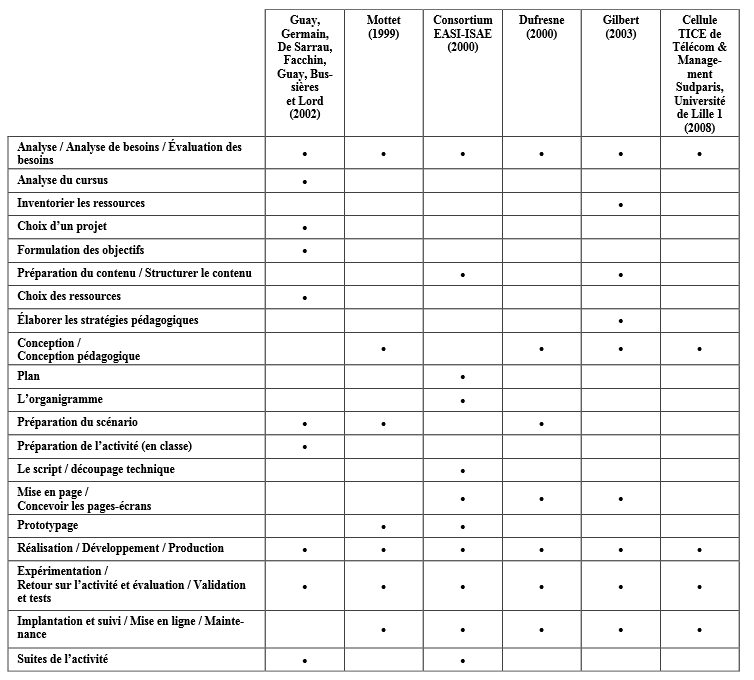
\includegraphics[width = 0.45\textwidth]{tableau6methodes.png}
                     \caption{\tiny{Tableau comparatif des étapes de six méthodes utilisées pour la conception et la réalisation d’outils pédagogiques en ligne \citep[p.20]{bonneau2013a}}}
                   \end{figure}
                   \begin{itemize}                   
                   \item On constate donc qu’il y a une \textbf{grande disparité} entre les méthodes et que, comme le dit \citet{bonneau2013a}, peu font l’unanimité ;
                   \item La variété des méthodes pourrait s’expliquer par le fait que les \textbf{outils pédagogiques en ligne sont protéiformes}, c’est-à-dire qui peut prendre diverses formes ;
                   \item Il faut donc demeurer\textbf{ critiques sur l’application d’un processus systématique} ;
                   \item \citet[p.10]{retalis1997a}, \citet[p.46]{smith2006a} et \citet[p.3]{pohl2004a} le confirment.
                   \end{itemize}
			\par \citet[p.3]{pohl2004a} prétend que : 
			\par« Guidelines for the development of e-learning systems have advantages and disadvantages. One disadvantage is that it is sometimes difficult to generalize guidelines. Related to that is the fact that the efficiency of educational media \textbf{always depends on the context} in which they are used. Guidelines should, therefore, not be formulated as cookbook recipes but rather be \textbf{flexible tools which can be adapted to various different situations and environments}. If such a flexible approach is used, guidelines can be applied quite effectively ».
			\par  Il a donc fallu prévoir, lors du survol, traiter de l’aspect de la situation de travail: soit du \textbf{contexte dans le cadre duquel les processus sont utilisés.}
                \end{frame}

\subsection{Milieu et les personnes concernées} 
		\begin{frame}[allowframebreaks]
			\frametitle{Précision sur le milieu et les personnes concernées}
                        \
                        \begin{itemize} 
                        \item  Les équipes sont \textbf{multidisciplinaires} ;
                        \item Ces équipes sont formées de : 
                        	\begin{itemize}
                        		\item concepteur pédagogique / conseillers pédagogiques ou technopédagogiques,
                        		\item intégrateurs, les infographistes, les programmeurs, les spécialistes des réseaux,
                        		\item de chargés de projets ou gestionnaires dirigent les projets.
                        	\end{itemize}

                        \end{itemize}

             
                \end{frame}

\subsection{La nécessité} 
		\begin{frame}[allowframebreaks]
			\frametitle{La nécessité d’un survol}
                        
                        \begin{itemize} 
                        \item  \textbf{Les méthodes }dans le domaine de la conception et de la réalisation d’outils pédagogiques en ligne \textbf{sont importantes.} \citet[p. 842]{bohl2002a}, \citet[p. 218]{barry2003a}, \citet[p. 1]{hadjerrouit2007a} tirés de \cite{bonneau2013a} le confirment;
                        \item La conception et la réalisation d’outils pédagogiques en ligne s\textbf{ont souvent faites par des novices en la matière} \citep[p. 351]{verstegen2008a} tiré de \citet{bonneau2013a};
                        \item Les enseignants semblent avoir une \textbf{vision restreinte au niveau de l’ampleur et de la complexité} (voire l’entièreté des problèmes) que l’appropriation d’une telle pratique peut créer, soit une vision générale de tout le processus engendré par une telle démarche dans un dispositif de FAD \citep[p. 105]{roy2011a} tiré de \citet{bonneau2013a}; 
                        \item Les méthodes d’ingénierie pédagogique comme la \textbf{méthode ADDIE, auraient provoqué une simplification de la perception} qu’ont de nombreux acteurs du domaine de l’éducation de ce processus\citep[p.28]{bonneau2013a} ;
                        \item \textbf{En récupérant une méthode d’ingénierie pédagogique pour en faire une méthode de conception et de réalisation d’outil pédagogique en ligne, on propage l’idée que ce processus est simple, pour ne pas dire simpliste\citep[p.29]{bonneau2013a} ;}
                        \item Il y aurait peut-être nécessité d'une d’une \textbf{méthode synthèse issue des travaux de recherche et de ce qui se fait dans la réalité.}

                        \end{itemize}

             
                \end{frame}
                
                \subsection{Objectif général} 
		\begin{frame}
			\frametitle{Objectif général}
                        
                        \begin{itemize} 
                        \item  Quels sont les situations de travail, les processus de production, du contrôle de la qualité et de bonnes pratiques en conception et réalisation d’outil pédagogique en ligne dans le milieu des producteurs d’outil pédagogique en ligne québécois, et ce pour la plupart des milieux soit la FGJ, FGA, FP, le CÉGEP, l’université et l’entreprise privée? 
                         \item Quelles sont les voies à privilégier afin d’améliorer les failles notées et rendre ce travail plus efficient?

                        \end{itemize}

             
                \end{frame}
                
	\section{Méthodologie} 
		
                        
				\subsection{Type de recherche} 
					\begin{frame}
						\frametitle{Type de recherche}
                        
                        			\begin{itemize} 
                       				 \item \textbf{Étude de 6 cas de producteurs d’outil pédagogique en ligne.} 
                       				 %\item Travail d’analyse par théorisation ancrée 
                       				 %\item Codification, catégorisation et mise en relation 

                       		 \end{itemize}
				\end{frame}
                       	\subsection{Déroulement de la recherche} 
					\begin{frame}[allowframebreaks]
						\frametitle{Déroulement de la recherche}
                        
                        			\begin{itemize} 
                       				 \item \textbf{Recensement normes et standards} de qualité en e-learning (non traité) ;
                       				 \item \textbf{Entretiens} avec des producteurs d’outil pédagogique en ligne font partie de l’échantillon ; 
                       				 \item Les \textbf{notes}, \textbf{traces documentaires} et \textbf{verbatim} de ces entretiens servent de matières premières à la recherche  ;
                       				 \item Analyse en profondeur :
                       				 \begin{itemize} 
                       				 	\item des situations de travail, 
                       				 	\item des processus de production,
                       				 	\item du contrôle de la qualité,
                       				 	\item des bonnes pratiques.
                       				 \end{itemize}
                       				 %\item Élaboration de la typologie qui permet de :
                       				 %\begin{itemize} 
                       				 	%\item nommer,
                       				 	%\item regrouper 
                       				 	%\item hiérarchiser les différentes étapes des méthodes étudiées,
                       				 	%\item validation de la typologie par des experts, 
                       				 	%\item élaboration des matrices de comparaison.
							%\end{itemize}
                       		 \end{itemize}

             
                \end{frame}
                     	\subsection{Population à l’étude} 
					\begin{frame}[allowframebreaks]
						\frametitle{Population à l’étude}
                        
                        			\begin{itemize} 
                       				 \item La population cible est constituée de \textbf{6 producteurs d’outil pédagogique }en ligne ;										 \item L’échantillon est le plus grand possible dans les limites et les contraintes financières ; 
                       		              \item L’ensemble des interviews a produit :
                       		              \begin{itemize} 
                       		              	\item 10 heures d’entretien,
                       		              	\item plus de 350 pages de verbatim,
                       		              	\item plus de 20 documents de traces.
                       		              \end{itemize}
                       		 \end{itemize}
                       		 \end{frame}
				\subsection{Critères de sélection} 
					\begin{frame}[allowframebreaks]
						\frametitle{Critères de sélection}
                        
                        			\begin{itemize} 
                       				\item Être disponibles.
							\item Provenir :
							\begin{itemize}
								\item de l’entreprise, 
								\item de la formation générale des jeunes, de la formation générale des adultes ou de la formation professionnelle, 
								\item du CÉGEP, 
								\item de l’université 
								\item de l’entreprise privée.
							\end{itemize}
							\item Avoir des petites organisations proches des enseignants comme des grandes organisations ayant de grosses équipes de production.
                       		 \end{itemize}
                       		 \end{frame}
                       		 \subsection{Échantillon} 
					\begin{frame}[allowframebreaks]
						\frametitle{Échantillon}
                        
                        			\begin{itemize} 
                       				\item Producteur 1 : un CÉGEP produisant des outils pédagogiques en francisation encadrés par le Ministère de l’Immigration de la Diversité et de l'Inclusion ;
                       				\item Producteur 2 : une microentreprise produisant des outils pédagogiques pour les entreprises et expertes dans l’accompagnement des organismes dans les étapes de préproduction ;
							\item Producteur 3 : un partenariat public privé producteur d’outils pédagogiques en ligne pour la formation générale des jeunes et la formation générale des adultes ;
							\item Producteur 4 : une PME produisant des outils pédagogiques en ligne pour des entreprises et des organismes publics ;
							\item Producteur 5 : un centre de formation professionnelle producteur d’outils pédagogiques pour une attestation de spécialisation professionnelle (ASP) encadrée par le MEESR ;
							\item Producteur 6 : une grande université produisant des outils pédagogiques en ligne pour plusieurs programmes d’études ou cours en ligne.

                       		 \end{itemize}
                       		           
                \end{frame}
                       		 
                       		 \subsection{Les techniques et instruments de collecte de données} 
					\begin{frame}[allowframebreaks]
						\frametitle{Les techniques et instruments de collecte de données}
                        
                        			\begin{itemize} 
                       				\item \textbf{L’approche semi-dirigée} a d’abord été utilisée afin de mieux comprendre :
                       				\begin{itemize}
                       				 	\item les processus de production, 
                       				 	\item le contrôle de la qualité ,
                       				 	\item les bonnes pratiques.
                       				 \end{itemize}
                       				\framebreak
                       				\item \textbf{L’approche dirigée} a été utilisée afin de mieux comprendre :
                       				\begin{itemize}
                       					\item les situations de travail,
                       					\item les demandes et les attentes,
                       					\item écarts entre la tâche telle que prévue et l’activité réelle de travail,
                       					\item bilan des difficultés rencontrées conséquences possibles du travail.
							\end{itemize}
							\item Une \textbf{grille préliminaire d’analyse} lors des entretiens
							\item \textbf{Analyse des traces} (des documents pertinents à la compréhension)
							\item Des \textbf{enregistrements sonores} ont été produits lors des entretiens
							\item Les \textbf{enregistrements sonores} ont été transcrits sous forme de verbatim qui ont été analysés à l’aide du logiciel nVivo
                       		 	\end{itemize}
                       		           
                			\end{frame}
                
                  \section{Résultats} 
                  %\subsection{Normes de qualité} 
					%\begin{frame}[allowframebreaks]
						%\frametitle{Recension des normes de qualité en production d’outils pédagogiques en ligne}
                        %La recherche documentaire démontre qu’il existait 3 grandes catégories de normes. 
                        			%\begin{itemize} 
                       				%\item Outils de contrôle de la qualité de l’éducation,
                       				%\item Normes technologiques en e-learning. 
                       				%\item Normes de qualité dédiées à l’e-learning.
                       		 	%\end{itemize}
                       		 %\end{frame}                   
                  %\subsection{Outils de contrôle de la qualité de l’éducation} 
					%\begin{frame}[allowframebreaks]
						%\frametitle{Outils de contrôle de la qualité de l’éducation}
                        			%\begin{description}[Second Item]
							
							%\item[Chartes] est un outil déontologique.
							%\begin{itemize}
								%\item Elle ne comporte pas de critère mesurable
								%\item Elle énonce des engagements du fournisseur envers ses clients.
							%\end{itemize}
							
							%\framebreak
							
							%\item[Labels] engagent une tierce partie dans la relation qui unit le client à son fournisseur. 
							%\begin{itemize}
								%\item Ils sont accordés par un organisme extérieur à l’organisme de formation. 
								%\item Ne concernent pas le contenu des formations. 
								%\item Une démarche commerciale 
								%\item Exemple, au Canada: Red Flag ou le CPMT
							%\end{itemize}
							
							%\framebreak
							
							%\item[Certifications] de tierces parties accréditées, il y en a deux types :
							%\begin{itemize}
								%\item certifications de services : 
								%\begin{itemize}
									%\item nécessité d’un éclaircissement dans le domaine des services, en l’absence de sigle officiel en guise de qualité
									%\item exemple 1 : les différents cadres de référence produits par le MEESR servent de certification de service au Québec, 
									%\item exemple 2 :  en France, un organisme indépendant produit ces certifications de services, il s’agit de l’AFNOR ;
								%\end{itemize}
								
								%\framebreak
								
								%\item standards d'assurance qualité :
								%\begin{itemize}
								%\item posent des principes de management,
								%\item  s’appliquent à tous les secteurs d’activité de façon non spécifique,
								%\item décrivent une organisation interne, propre à chaque organisation,
								%\item visent à minimiser les risques de dysfonctionnement grâce à l’application de procédures,
								%\item contrat transparent avec le client ou l’a, qui peut être l’apprenant
								%\item exemple 1: En mai 2000, 250 organismes ayant pour activité principale la formation professionnelle avaient été certifiés par la norme ISO 9001-1994 en France.
								%\item exemple 2 :  Au Québec, les normes de qualité ISO sont peu adoptées en éducation et en formation continue, même sur le plan des entreprises. Selon le BNQ , 2 organismes publics étaient certifiés ISO9001 en 2015 , et 1 entreprise de formation.
								%\end{itemize}
								   
							%\end{itemize}
						
						%\framebreak
						
						%\item[Technologiques] Il existe une grande variété de standards techniques :  
							%\begin{itemize}
							%\item beaucoup sont de l’ordre de la structuration et de la description des métadonnées, 
							%\item d’autres sont pour les paquetages de cours (SCORM, AICC, etc.),
							%\item il s’agit de spécifications techniques, 
							%\item bien qu’elles soient utilisées par nos producteurs, il ne s’agit pas, dans le cadre de ce travail, de notre principal champ d’intérêt ;
							%\end{itemize}
						
						%\framebreak
						
						%\item[Dédiés] Parmi les normes de l'e-learning, nous comptons :
							%\begin{itemize}
							
							%\framebreak
							
							%\item QUALITÉ TOTALE  
								%\begin{itemize}
								%\item s’intéresse davantage à l’organisme d’e-learning que directement à ses clients
								%\item elle permet de promouvoir la gestion de la qualité au sein des organismes d’e-learning
								%\item elle permet de rechercher les bonnes pratiques dans une démarche d’auto-évaluation. 									
								%\framebreak
								
								%\item exemple : la SOFEDUC a écrit 10 normes qui s’intéressent :
								 	%\begin{itemize} 
								 	%\item au besoin de formation
								 	%\item aux objectifs d’apprentissage,
								 	%\item aux formateurs,
								 	%\item aux contenus des formations,
								 	%\item aux stratégies de formation,
								 	%\item à l’évaluation des apprentissages,
								 	%\item à l’évaluation de l’activité ou du programme de formation,
								 	%\item à l’unité responsable
								 	%\item au système d’amélioration continue,
								 	%\item aux dossiers des participants ;
								 	%\end{itemize}
								 %\end{itemize}
							
							%\framebreak
							
							%\item QUALITY STANDARDS FOR EVALUATING MULTIMEDIA AND ONLINE TRAINING  
								%\begin{itemize}
								%\item permet d’estimer comment un cours en ligne satisfait aux exigences fondamentales de la qualité dans chacun des quatre champs suivants : 
									%\begin{itemize}
									%\item les besoins organisationnels,
									%\item le contenu pédagogique,
									%\item la convivialité
									%\item l’architecture des instructions pour l’enseignement. 
									%\end{itemize}
								%\end{itemize}
							
							%\framebreak
							
							%\item QUALITY IN OPEN AND DISTANCE LEARNING, QUALITY CONCIL (ODL/QC) 
								%\begin{itemize}
								%\item complémentaire aux précédentes et s’intéresse à : 
									%\begin{itemize}
									%\item l’inscription et à l’accompagnement des élèves
									%\item l’environnement d’apprentissage
									%\item l’offre du fournisseur de ressources
									%\item aux clauses du contrat de formation. 
									%\end{itemize}
								%\item Il s’agit d’une accréditation qui peut être obtenue sur présentation d’un dossier et après
								 %une visite.	
								%\end{itemize}
							
							%\framebreak
							
							%\item DISTANCE LEARNING GUIDELINES 
								%\begin{itemize}
								%\item composée d’un ensemble de documents qui définissent les normes de qualité pour la conception du programme : 
									%\begin{itemize}
									%\item la prestation, 
									%\item l’accompagnement des apprenants, 
									%\item les modalités de communication avec l’apprenant,
									%\item l’évaluation de l’apprenant, 
									%\item le travail de groupe.
									%\end{itemize}
								%\end{itemize}
							
							%\framebreak
							
							%\item Autres normes
								%\begin{itemize}
								%\item ISTE : sert à préparer l’enseignant et l’apprenant au meilleur usage des technologies dans la nouvelle société de l’information
								%\item DITRA : est un programme de la communauté européenne plus particulièrement dédié à la construction de modèles de compétences requises par les acteurs de l’e-learning, dans les diverses étapes de sa conception et de son utilisation
								%\item GUIDE DES BONNES PRATIQUES POUR DÉVELOPPER LES COMPÉTENCES PAR LE NUMÉRIQUE DU CÉFRIO : qui est un survol des usages et bonnes pratiques pour les projets de formation avec le support des TIC. 
								%\item LABEL OPQF : est quant à lui attribué en reconnaissance du professionnalisme d’un produit, de ses compétences, et de l’expérience professionnelle dans un ou plusieurs domaines de qualification sélectionnés parmi les 19 domaines existants.
								%\end{itemize}
							%\end{itemize}						
						%\end{description}
		 %\end{frame}   
		 
		 \subsection{Acteurs} 
					\begin{frame}[allowframebreaks]
						\frametitle{Acteurs}
                        			\begin{figure}
                     			\centering
                    			 \includegraphics[width = 0.75\textwidth]{acteurs.png}
                     			\caption{\tiny{Schéma sur les acteurs produit pour la CSDL}}
                   			\end{figure}
                        			Nous avons tenté, pour chaque participant, de cerner les personnes ou organismes qui sont appelés à contribuer à la production d’un outil pédagogique en ligne.
							\begin{itemize}
							\item \textbf{Grandes variétés d'acteurs} ;
							\item Les acteurs sont de l'\textbf{interne} et de l'\textbf{externe} ;
							\item \textbf{Multidisciplainaire} :
								\begin{itemize}
								\item acteurs \textbf{recherche} : 
									\begin{itemize}
									\item CNT (conseiller en nouvelles technologies,
									\item Conseillère en recherche et développement (CRD) ;
									\end{itemize}
								\item acteurs\textbf{ techniques},												
								\item acteurs \textbf{pédagogiques} :
									\begin{itemize}
									\item contenu,
									\item conception pédagogique,
									\item conception technopédagogique,
									\item droits d'auteur,
									\item environnement numérique d'apprentissage ;
									\end{itemize}
								\item\textbf{ client :}
									\begin{itemize}
									\item apprenant,
									\item entreprises et OSBL, 
									\item Organismes publics comme clients (ministères, commissions scolaires, écoles et centres) ;
								\end{itemize}
								\item acteurs \textbf{créatifs} : 
									\begin{itemize}
									\item spécialistes du Web,
									\item spécialistes de l'image,
									\item spécialistes de l'audio,
									\item spécialistes de la vidéo,
									\item intégrateurs multimédia ;
									
									\end{itemize}
								\item \textbf{grands acteurs du Web : 	}	
									\begin{itemize}
									\item grands services infonuagiques tels que Google,
									\item réseaux sociaux ;
									\end{itemize}
								\item acteurs du \textbf{contrôle de la qualité} :
									\begin{itemize}
									\item réviseurs,
									\item testeurs, 
									\item responsable de la qualité.
									\end{itemize}
								\item acteurs en \textbf{gestion}.
								\end{itemize}
							\item La \textbf{démocratisation} des outils \textbf{diminue le nombre d'acteurs} ;
							\item La \textbf{complexité} des outils \textbf{augmente le nombre d'acteurs spécialisés} ;
							\end{itemize}
						
					\end{frame}
					
					
					
					 \subsection{Étapes de production}
					  
						\begin{frame}[allowframebreaks]
						\frametitle{Étapes de production}
						\begin{figure}
                     			\centering
                    			 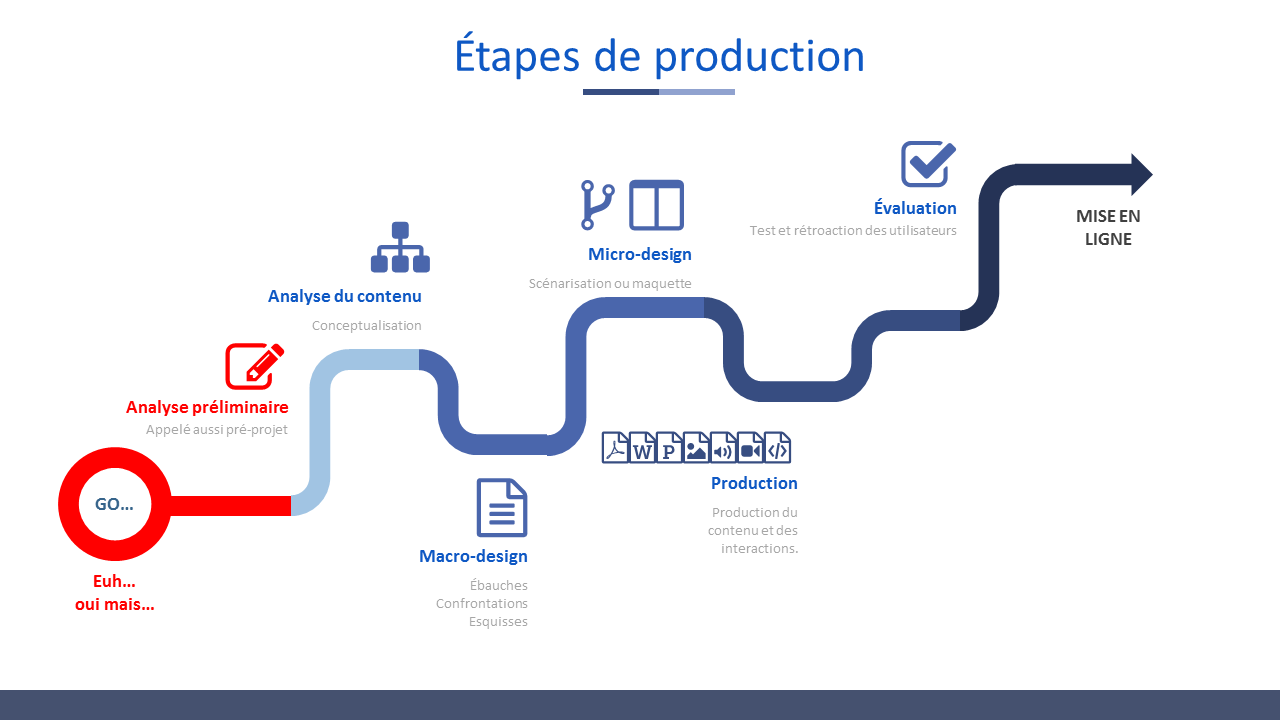
\includegraphics[width = 0.75\textwidth]{etapes.png}
                     			\caption{\tiny{Schéma synthèse sur les étapes de production produit pour la CSDL}}
                   			\end{figure}
                   			
                   			
                        			Nous avons tenté, pour chaque participant, de cerner l’ensemble des \textbf{phases nécessaires à la transformation des matières premières en produits finis.}
						\begin{itemize}
						\framebreak
						\item \textbf{Grandes variétés d'étapes} ;
						\item Les \textbf{organisations moins spécialisées} ont un \textbf{processus de production moins développé} ;
						\item Les \textbf{organisations moins spécialisées} n'ont \textbf{pas ou peu de processus l'analyse préliminaire} ;
						\item \textbf{Peu d'organisation} utilise des \textbf{méthodes de gestion de projet itératives} ou \textbf{organique };
						\item Les organisations spécialisées sont fortement influencées par l'ADDIE.
						\end{itemize}
						\framebreak
						Voici les principales étapes de production observées :	
						\begin{itemize}
						\item \textbf{avant le projet} : 
							\begin{itemize}
							\item \textbf{analyse préliminaire}, pré projet, avant-projet, analyse du besoin ou d'une problématique, première discussion, tempête d’idées, 
							\item test des dispositifs de la compétition, 
							\item \textbf{analyse du contenu} : modélisation de connaissances, inventaire de que le client détient déjà (contenu et matériel), définition des apprentissages doivent être produits,organisation du contenu d’apprentissage, etc.,
							\item \textbf{conception} :
								\begin{itemize}
								\item \textbf{production de documents} papier et  correction sur le matériel écrits,
								\item \textbf{prototypage}, esquisses, confrontation, ébauche, micro et macrodesign ;
								\end{itemize}
							\end{itemize}
						\framebreak
						\item \textbf{pendant le projet }:
							\begin{itemize}
							\item \textbf{production ou développement} :
								\begin{itemize}
								\item médiatisation,
								\item production des composantes,
								\item assemblage sur un environnement numérique d'apprentissage,
								\item tests,
								\end{itemize}
							\framebreak
							\item \textbf{implantation} :
								\begin{itemize}
								\item prétest, 
								\item prestation,
								\item évaluation des étudiants et du cours,
								\item post-prestation,
								\item archivage ;
								\end{itemize}
							\end{itemize}
						\framebreak
						\item \textbf{après le projet} : 
							\begin{itemize}
							\item \textbf{évaluation ou bilan et analyse de la prestation} :
								\begin{itemize}
								\item évaluation technique,
								\item test par des humains (enseignants, élèves, etc.),
								\item correction pour faire suite aux tests effectués par les élèves ;
								\end{itemize}
							\end{itemize}	
						\item \textbf{processus d'amélioration continue} (peu mentionné) :
								\begin{itemize}
								\item amélioration au cours du temps, 
								\item rencontre fréquentes.
								\end{itemize}
						\end{itemize}		
							
						
					\end{frame}
							
						
						 \subsection{Livrables} 
						\begin{frame}[allowframebreaks]
						\frametitle{Livrables}
						\begin{figure}
                     			\centering
                    			 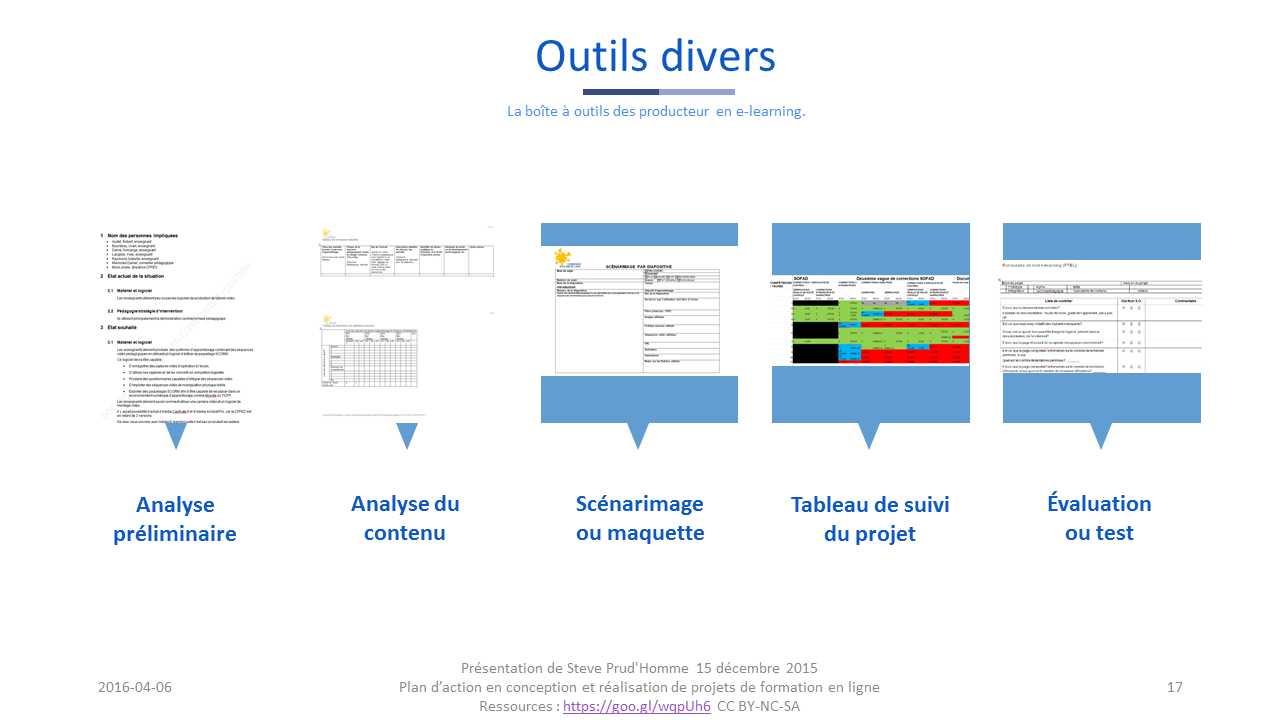
\includegraphics[width = 0.75\textwidth]{livrables1.png}
                     			\caption{\tiny{Schéma sur les livrables pédagogiques produit pour la CSDL}}
                   			\end{figure}
                   			\begin{figure}
                     			\centering
                    			 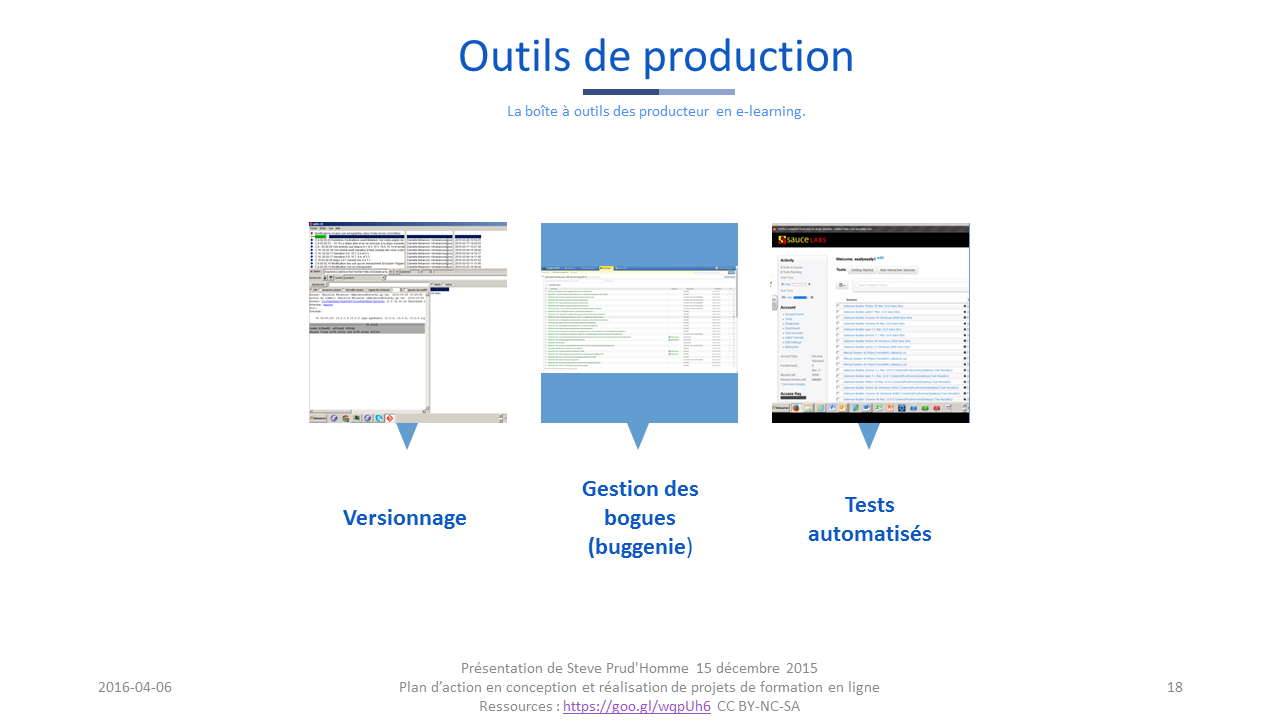
\includegraphics[width = 0.75\textwidth]{livrables2.png}
                     			\caption{\tiny{Schéma sur les livrables techniques produit pour la CSDL}}
                   			\end{figure}
                   			
                        			Nous avons tenté, pour chaque participant, de cerner l’ensemble des \textbf{résultats attendus dans le cadre d’un projet d’outils pédagogiques en ligne et qui seront matérialisés par un produit, un document de référence ou une activité.}
						\begin{itemize}
							\item \textbf{Grande variété de livrables ;}
							\item Les o\textbf{rganisations moins spécialisées focalisent} sur les \textbf{outils pédagogiques en lignes finaux };
							\item Les \textbf{organisations plus spécialisées mettent plus d'emphase} sur les \textbf{livrables de planification} comme l'\textbf{analyse préliminaire} ou l'\textbf{analyse du contenu} ;
							\item Les \textbf{organisations moins spécliasées substituen}t ce qui est fait dans la classe.
						\end{itemize}		
						Nous avons observé 8 types de livrables.
						
						
					\end{frame}

						\subsubsection{Livrables de planification} 
							\begin{frame}[allowframebreaks]
							\frametitle{Livrables de planification}
                        		Souvent sous la forme d'une analyse d’affaire, d'un préprojet, d'un \textbf{rapport d’analyse préliminaire}, tableau de spécification de la conception, etc.
	
							\begin{itemize}
							\framebreak
							\item \textbf{Analyse préliminaire} :
								\begin{itemize}
								\item situation :
									\begin{itemize}
									\item \textbf{généralités} : objectifs de la campagne de production du projet, identification, présentation ou description du projet, de ce qui sera produit et objet du projet, 
									\item \textbf{besoins }: provenance de la demande et nombre d’heures,
									\item \textbf{clientèle visée},
									\item \textbf{impact} : impacts prévus et résultats attendus,
									\item \textbf{risques }: identification et évaluation des éléments de risque et de complexité et faisabilité de projet,										
									\item \textbf{étude du marché} : Marché et concurrence prévus ;								
									\end{itemize}
								\framebreak
								\item \textbf{exécution} : 
									\begin{itemize}
									\item \textbf{échéanciers} ;
									\end{itemize}
								\item \textbf{administration et logistique} :
									\begin{itemize}
									\item \textbf{finance} (Modalités de financement et partenariat possibles),						
									\item présentation et disponibilités des auteurs et des collaborateurs,
									\item ressources techniques et autres collaborations prévues à l’interne et approbation,
									\item ressources requises versus calendrier de réalisation ;
									\end{itemize}
								\end{itemize}
							\framebreak
							
							\item \textbf{Analyse du contenu} : 
								\begin{itemize}
								\item \textbf{contenu }: 
									\begin{itemize}
									\item élaboration, conception du cours, objectifs et activités d’apprentissage, matrice des apprentissages,
									\item matériels existants réutilisables (documents existants, droits d’auteurs, etc.),
									\item objectifs/contenus/compétences (programmes existants ou à élaborer),
									\item rapport de recherche ou de veille, 
									\item \textbf{analyse de contenus }: modèle des connaissances, liens typés, grammaire, etc. : représentation graphique des connaissances faites avec le titulaire ;
									\end{itemize}
								\item \textbf{clientèle cible} :
									\begin{itemize}
									\item objectifs de la clientèle du cours ;
									\end{itemize}
								\item \textbf{ressources} : 
									\begin{itemize}
									\item demandes de droit d’auteur, 
									\item impact du choix des ressources ;
									\end{itemize}
								\item \textbf{bibliographies}
									\begin{itemize}
									\item bibliographies, recensement et sélection des ressources existantes,
									\item ressources bibliographiques et collections savantes ;
									\end{itemize}
								\end{itemize}
							\item \textbf{Autres livrables} : 
								\begin{itemize}
								\item vision institutionnelle,
								\item contrats types,
								\item devis,
								\item proposition,
								\item cahier des charges, 
								\end{itemize}
							\framebreak
							\end{itemize}	
												
					\end{frame}

						\subsubsection{Livrables de conception} 
							\begin{frame}[allowframebreaks]
							\frametitle{Livrables de conception}
                        			
							\begin{itemize}
							\item \textbf{Macrodesign} : 
								\begin{itemize}
								\item structure, métaphore, comment le dispositif de formation est organisé,
								\item description et justification des médias et des choix technologiques ;
								\end{itemize}
							\item \textbf{Microdesign} :
								\begin{itemize}
								\item scénarisation : 
									\begin{itemize}
									\item scénario : découpage de la formation,
									\item scénarimage ;
									\end{itemize}
								\item document de planification détaillée,
								\item table des matières,
								\item maquettes,
								\item ébauches.
								\end{itemize}								
							\end{itemize}						
					\end{frame}
					
					
					\subsubsection{Livrables de production} 
							\begin{frame}
							\frametitle{Livrables de production}
                        			
							\begin{itemize}
							\item \textbf{Charte graphique} :
								\begin{itemize}
								\item production de l’image institutionnelle,
								\item production des feuilles de styles ;
								\end{itemize}
							\item \textbf{Gabarits} :
								\begin{itemize}
								\item gabarit de cours qui inclut une charte graphique,
								\item ressources et gabarit génériques ;
								\end{itemize}
							\item Production des \textbf{ressources communes} ;
							\item Lignes directrices par rapport, aux fichiers multimédias.
						
							\end{itemize}						
					\end{frame}
					
						\subsubsection{Livrables de prototype} 
							\begin{frame}
							\frametitle{Livrables de production}
                        			
							\begin{itemize}
							\item \textbf{Prototype} (\textit{staging}) : produit pilote pour la validation du client et demande de non-conformité.
						
							\end{itemize}						
					\end{frame}
					
					\subsubsection{Livrables liés au produit final} 
							\begin{frame}[allowframebreaks]
							\frametitle{Livrables liés au produit final}
                        			
							\begin{itemize}
							\item Interface ;
							\item Documentation: technique et utilisateur :
								\begin{itemize}
								\item procéduriers élèves,
								\item documentation et textes d’aide ;
								\end{itemize}
							\item Cours complets :
								\begin{itemize}
								\item activités:
									\begin{itemize}
									\item liens URL,
									\item PDF,
									\item tests,
									\item \textbf{capsules interactives},
									\item autres activités pédagogiques (ex.: glossaire, etc.).
									\end{itemize}
								\framebreak
								\item ressources ;
									
								\end{itemize}
							\item \textbf{Documents d'accompagnement} :
								\begin{itemize}
								\item cahiers d’exercices (textes),
								\item feuilles de route,
								\item horaires.
								\end{itemize}
							\end{itemize}						
					\end{frame}
					
					\subsubsection{Livrables liés au contrôle de la qualité} 
							\begin{frame}[allowframebreaks]
							\frametitle{Livrables liés au contrôle de la qualité}
                        			
							\begin{itemize}
							
							\item \textbf{Tests} : 
								\begin{itemize}
								\item tests automatisés,
								\item tests unitaires,
								\item tests d’intégration ;
								\end{itemize}
							\item Approbations :
								\begin{itemize}
								\item formulaires électronique et approbation de la direction,
								\item formulaire de mise en ligne et approbation de la direction ;
								\end{itemize}
							\item Appréciation : 
								\begin{itemize}
								\item \textbf{formulaire d’appréciation d’un cours} ;
								\end{itemize}
							\framebreak
							\item Audits de médias sociaux ;
							\item \textbf{Rapports liés au contrôle de la qualité} :
								\begin{itemize}
								\item documentation du contrôle de la qualité en ce qui concerne l’aspect technique,
								\item résultats de tests,
								\item rapport d’interprétation des appréciations des élèves ,
								\item document de rapport final.
								
								
								\end{itemize}
							\end{itemize}						
					\end{frame}

					\subsubsection{Livrables liés aux données} 
							\begin{frame}
							\frametitle{Livrables liés aux données}
                        			
							\begin{itemize}
							
							\item Données sur évaluation pédagogique ;
							\item \textbf{Profil pédagogique complet d’un étudiant };
							\item Information et données sur les différents aspects du dispositif de formation.
								
							\end{itemize}						
					\end{frame}
					
					\subsubsection{Livrables liés à l'implantation} 
							\begin{frame}
							\frametitle{Livrables liés à l'implantation}
                        			
							\begin{itemize}
							
							\item Cahier d’exploitation ; 
							\item Plan de transition.
								
							\end{itemize}						
					\end{frame}
					
					
				\subsection{Contrôle de la qualité} 
						\begin{frame}[allowframebreaks]
						\frametitle{Contrôle de la qualité}
                        			\begin{figure}
                     			\centering
                    			 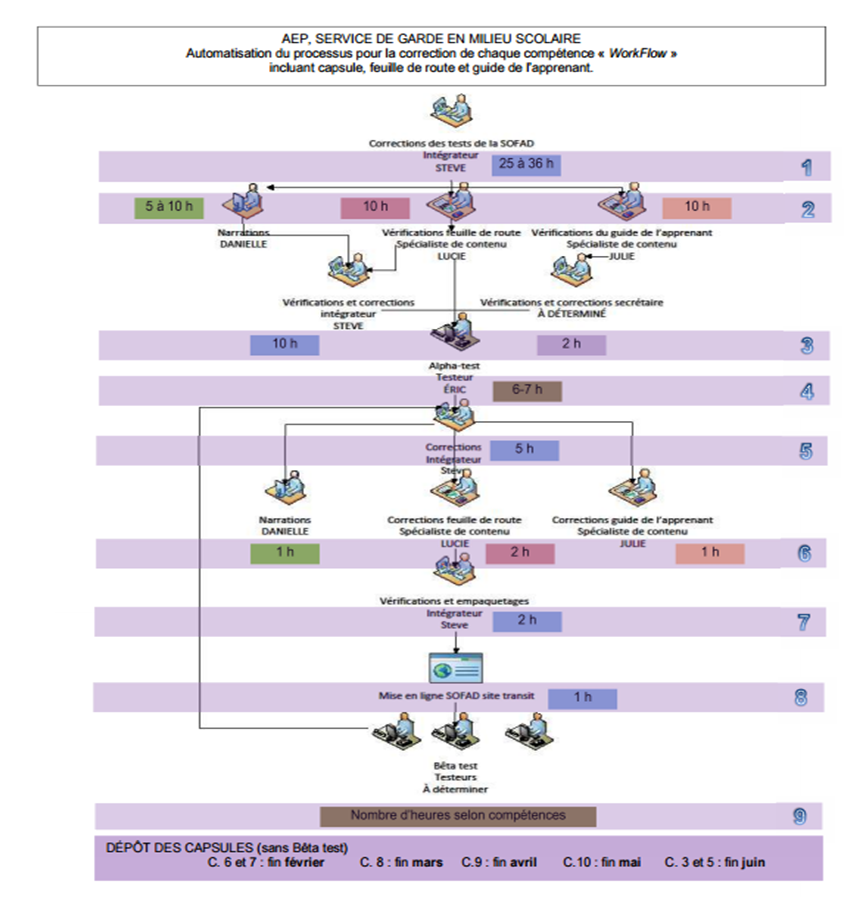
\includegraphics[width = 0.30\textwidth]{flux.png}
                     			\caption{\tiny{Flux de production élaborée pour l'AEP service de garde CSDL}}
                   			\end{figure}
                        			Nous avons tenté, pour chaque participant, de cerner les \textbf{moyens ou procédures mis en œuvre afin de vérifier la conformité d’un outil pédagogique en ligne à des \textit{normes de qualité} déterminées ou pas.}
						
						\end{frame}
						
					\subsubsection{Contrôle de la qualité lors de l'analyse préliminaire} 
							\begin{frame}
							\frametitle{Contrôle de la qualité lors de l'analyse préliminaire}
                        				
							\begin{itemize}
							
							\item Notes, cahier de notes, relecture des notes qui augmentent la précision ;
							\item Lecture préliminaire du client. 
												
							\end{itemize}						
					\end{frame}	
					\subsubsection{Contrôle de la qualité : modélisation} 
							\begin{frame}[allowframebreaks]
							\frametitle{Contrôle de la qualité : modélisation}
                        			
							\begin{itemize}
							\item Méthode Mot.
							\end{itemize}						
					\end{frame}	
					
					\subsubsection{Contrôle de la qualité : outils de production} 
							\begin{frame}
							\frametitle{Contrôle de la qualité : outils de production}
                        			
							\begin{itemize}
							
							\item Coquilles vides ou \textbf{gabarits} ;
							\item \textbf{Charte graphique} ;
							\item Les \textbf{lignes directrices} par rapport aux formats de fichiers multimédias.
												
							\end{itemize}						
					\end{frame}	
					\subsubsection{Contrôle de la qualité : utilisation de l'environnement numérique d'apprentissage} 
							\begin{frame}
							\frametitle{Contrôle de la qualité : utilisation de l'environnement numérique d'apprentissage}
                        			
							\begin{itemize}
							\item L’utilisation d'un environnement numérique d'apprentissage permet de savoir à tout moment, en tant qu’administrateur, qui est connecté, qui fait quoi ;
							\item Utilisation de fonction de l'environnement numérique d'apprentissage ce qui permet d’assurer d’avoir le contrôle de ce qui est fait de ce qui est diffusé aux étudiants.
							\end{itemize}						
					\end{frame}	
					\subsubsection{Contrôle de la qualité : utilisation des tests} 
							\begin{frame}
							\frametitle{Contrôle de la qualité : utilisation des tests}
                        			
							\begin{itemize}
							\item Période d’essais, de tentatives ;
							\item Expérimentation des produits (s’il y a lieu) ;
							\item Mise à l’essai du  prototype ;
							\item Tests techniques :
								\begin{itemize}
								\item \textbf{Test automatisé } avec des solutions logiciels telles que la suite Selenium et SauceLab,
								\item Test unitaire (ex. : authentification ou création d’un profil),
								\item Test d’intégration (comment interagissent les classes entre elles) ;
								\end{itemize}
							\item Tests pédagogiques :
								\begin{itemize}
								\item \textbf{Test pédagogiques unitaires} :  petit test sur les ressources. Par exemple, est-ce que cette séquence vidéo fonctionne ?
								\end{itemize}
							\item Utilisation d’une plateforme de test ;
							\item Test fait par un groupe (5 à 10 personnes) ;
							\item Formulaire de test de 5 à 10 questions.
							\end{itemize}						
					\end{frame}
						
					\subsubsection{Contrôle de la qualité : utilisation des élèves ou étudiants} 
							\begin{frame}
							\frametitle{Contrôle de la qualité : utilisation des élèves ou étudiants}
                        			
							\begin{itemize}
							
							\item \textbf{Rétroaction des étudiants} ;
							\item Appréciation des élèves, génération automatique de statistiques sur l’appréciation des élèves  ;
							\item Test avec certains élèves (plusieurs itérations) : la \textbf{recherche des coquilles }éventuelles et la correction des textes.										
							\end{itemize}						
					\end{frame}	
					
					\subsubsection{Contrôle de la qualité : utilisation des spécialistes de contenu} 
							\begin{frame}
							\frametitle{Contrôle de la qualité : utilisation des spécialistes de contenu}
                        			
							\begin{itemize}
							
							\item Utilisation de \textbf{multiples spécialistes de contenu} ;
							\item \textbf{Recherche des coquilles} éventuelles et la correction des textes ;
							\item Test entre enseignants ;
							\item Sollicite l’accord du professeur responsable (université).
							\end{itemize}						
					\end{frame}	
					
					\subsubsection{Contrôle de la qualité : utilisation des gestionnaires} 
							\begin{frame}
							\frametitle{Contrôle de la qualité : utilisation des gestionnaires}
                        			
							\begin{itemize}
							\item Approbation de la planification détaillée par la direction (direction générale et direction de projet) ;
							\item Les objectifs d’un cours en ligne établis par le chargé de projet en collaboration avec l’auteur sont approuvés par le directeur de projet ou de production ;
							\item La direction approuve la planification détaillée d’un projet ;
							\item Le directeur de projet ou de production donne son approbation en ce qui concerne les différents livrables
							\item \textbf{Tout ce qui est fait par les auteurs est validé par les chargés de projet} ;
							\item \textbf{Dépôt d’un premier chapitre et approbation} ;
							\item Dépôt de la production et approbation.
							\end{itemize}						
					\end{frame}	
					
					\subsubsection{Contrôle de la qualité : réviseurs} 
							\begin{frame}[allowframebreaks]
							\frametitle{Contrôle de la qualité : réviseurs}
                        			
							\begin{itemize}
							\item Lecture d’épreuves ;
							\item \textbf{Révision linguistique,  visuelle et révision des contenus}.
							
							\end{itemize}						
					\end{frame}	
					\subsubsection{Contrôle de la qualité : responsable de la qualité} 
							\begin{frame}[allowframebreaks]
							\frametitle{Contrôle de la qualité : réviseurs}
                        			
							\begin{itemize}
							\item Il y a des employés responsables de l’assurance qualité des cours (rare).
							\end{itemize}						
					\end{frame}	
					\subsubsection{Contrôle de la qualité : ministère} 
							\begin{frame}[allowframebreaks]
							\frametitle{Contrôle de la qualité : ministère}
                        			
							\begin{itemize}
							\item Les normes ministérielles (MEESR) agissent comme normes minimales de qualité.
							\end{itemize}						
					\end{frame}	
					\subsubsection{Contrôle de la qualité : le client} 
							\begin{frame}[allowframebreaks]
							\frametitle{Contrôle de la qualité : le client}
                        			
							\begin{itemize}
							\item Le client consulte l’épreuve sur un serveur de \textit{stagging}.
							\end{itemize}						
					\end{frame}	
					
					\subsubsection{Contrôle de la qualité : certification du personnel} 
							\begin{frame}[allowframebreaks]
							\frametitle{Contrôle de la qualité : certification du personnel}
                        			
							\begin{itemize}
							\item Certification PMP.
							\end{itemize}						
					\end{frame}	
								
				\subsection{La situation de travail} 
						\begin{frame}[allowframebreaks]
						\frametitle{La situation de travai}
                        			\begin{figure}
                     			\centering
                    			 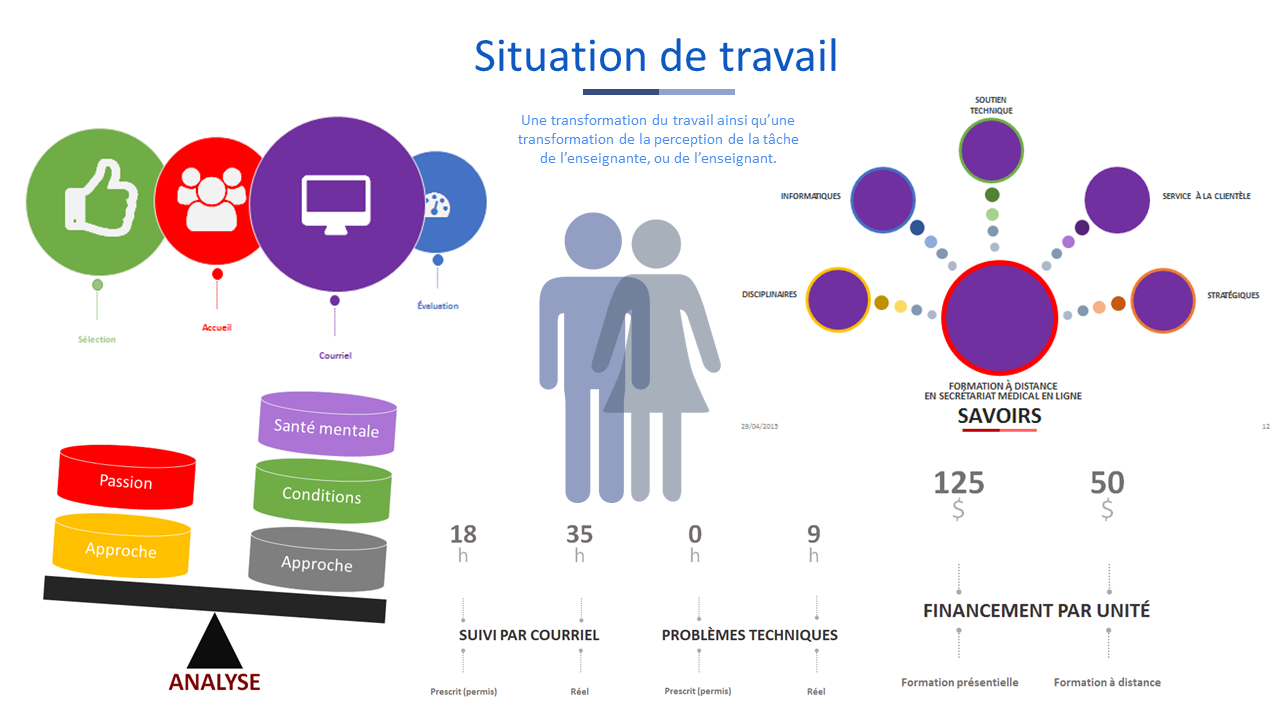
\includegraphics[width = 0.75\textwidth]{situation.png}
                     			\caption{\tiny{Schéma sur la situation de travail cours FPT7757 analyse ergonomique en FP}}
                   			\end{figure}
                        			Ce survol démontre que les producteurs de ressources pédagogiques en ligne devaient \textbf{faire face à plusieurs défis}. 
						
						\end{frame}	
													
				\subsubsection{Valorisation de la technopédagogie} 
						\begin{frame}[allowframebreaks]
						\frametitle{Valorisation de la technopédagogie}
                        			
                        			\begin{itemize}
                        			\item Les producteurs doivent \textbf{faire la promotion des TICE} auprès du monde de l’éducation
                        			\item Les technologies ne sont \textbf{pas connues} ou très mal connues par le monde de l’éducation. 
                        			\item \textbf{Le métier de technopédagogue est un métier méconnu et qui n’est pas mis en valeur. }
                        			\item \textbf{Les organisations}, parce que les technopédagogues et la technopédagogie sont mal connus, \textbf{prennent des raccourcis à cause du manque de connaissances}. 
                        			\item Certains participants ont exprimé comment le monde de l’éducation serait lourd, c’est-à-dire que, pour plusieurs, \textbf{le monde de l’éducation serait une grosse machine où les changements sont difficiles à apporter. }
                        			\item \textbf{Le monde de l’éducation poserait peu de questions et prendrait peu de risques.} 
                        			\item Beaucoup rapportent les \textbf{contraintes budgétaires qui seraient de plus en plus présentes} dans les organisations québécoises. 
						\end{itemize}
						
						\end{frame}	
						
					\subsubsection{Valorisation de l'éducation dans l'entreprise privée} 
						\begin{frame}[allowframebreaks]
						\frametitle{Valorisation de l'éducation dans l'entreprise privée}
                        			
                        			\begin{itemize}
                        			\item Beaucoup d’organisations et de gestionnaires accorderaient peu ou pas d’importance à l’éducation. 
                        			\item Beaucoup voudraient produire des producteurs et peu des penseurs. 
                        			
						\end{itemize}
						\end{frame}	
						
					\subsubsection{Perceptions de la formation en ligne en formation professionnelle} 
						\begin{frame}[allowframebreaks]
						\frametitle{Perception de la formation en ligne en formation professionnelle}
                        			
                        			\begin{itemize}
                        			\item \textbf{Les gestionnaires auraient très peu de connaissances} sur la formation en ligne et une \textbf{fausse conception} de celle-ci. 
                        			\item Les gestionnaire penseraient que la formation en ligne permettrait aux individus de faire leur formation seule sans support et sans contrôle de la qualité. 
                        			\item \textbf{Les gestionnaires mettraient même en doute l’immense travail fait par les enseignants ou membres des équipes de production}, surtout au niveau du suivi pendant la formation.
                        			\item Les gestionnaires penseraient que\textbf{ la formation en ligne peut sauver des programmes en baisse de clientèle ou en essoufflement}. 
                        			\item Le \textbf{mode de financement en formation à distance serait, médiocre.} En effet, dans le cas de métier de type administratif, 50 \$ par unité en formation à distance seraient accordés contre 120 \$ en formation traditionnelle. 
                        			\item Dans certaines industries, l’opinion des travailleurs par rapport à la formation à distance serait mitigée. \textbf{Certains auraient la perception qu’un travailleur formé à distance aurait suivi un cours de moindre qualité.}
                        			
						\end{itemize}
						\end{frame}	
						
					\subsubsection{Transformation du métier de l'enseignant} 
						\begin{frame}[allowframebreaks]
						\frametitle{Transformation du métier de l'enseignant}
                        			
                        			\begin{itemize}
                        			\item Passer du paradigme de l’enseignant-pourvoyeur de savoirs à l’\textbf{enseignant en e-learning spécialisé en :}
                        				\begin{itemize}
                        				\item suivi des dossiers d’élèves, 
                        				\item en service à la clientèle et 
                        				\item responsable du soutien technique 
                        				\end{itemize}
                        			\item L’enseignant serait appelé à :
                        				\begin{itemize}
                        				\item jouer un rôle différent, 
                        				\item développer des compétences qui ne sont pas traditionnellement associées au métier d’enseignant : 
                        					\begin{itemize}
                        					\item les compétences liées à l’utilisation de l’informatique
                        					\item le service à la clientèle, 
                        					\item le soutien technique, 
                        					\item les stratégies de communication, 
                        					\item l’écoute active par téléphone ou courriel, etc. ;
                        					\end{itemize}
                        				\item \textbf {combiner les charges d’enseignant en formation à distance et d’enseignant en formation individuelle ou en présentielle.}
                        			\end{itemize}
						\end{itemize}
						\end{frame}		
					
					\subsubsection{Climat de travail} 
						\begin{frame}[allowframebreaks]
						\frametitle{Climat de travail}
                        			
                        			\begin{itemize}
                        			\item Il serait lourd de travailler avec des collègues qui ne sont pas motivés à travailler.
                        				
						\end{itemize}
						\end{frame}		
						
					\subsubsection{Éléments positifs de la production d’outil pédagogique en ligne} 
						\begin{frame}[allowframebreaks]
						\frametitle{Éléments positifs de la production d’outil pédagogique en ligne}
                        			Les professionnels de l'éducation aiment : 
                        			\begin{itemize}
                        			\item Avoir la possibilité de changer les choses ;
                        			\item Qu’on les écoute ;
                        			\item Qu’on leur donne une chance d’innover, 
                        			\item Qu’on reconnaisse leur expertise, 
                        			\item Voir la réussite d’un projet, 
                        			\item Se sentir utiles, 
                        			\item Ne pas travailler pour rien, 
                        			\item Voir la réussite et la continuité des élèves,
                        			\item Avoir de bonnes relations avec les divers acteurs
                        			\item \textbf{Travailler avec des gens qui croient encore à la mission de l’éducation ou encore travailler avec des gens passionnés par l’enseignement.}
                        				
						\end{itemize}
						\end{frame}		
						
					\subsubsection{Marge de manœuvre} 
						\begin{frame}[allowframebreaks]
						\frametitle{Marge de manœuvre}
                        			
                        			\begin{itemize}
                        			\item Il y a \textbf{peu de marge de manœuvre}. 
                        			\item Les budgets sont la principale source de ce problème. Les budgets étant serrés, les horaires le deviennent nécessairement, les participants ont donc de la difficulté à pouvoir s’adapter à différentes situations problématiques tant au niveau de la production qu’au niveau du soutien aux apprenants.
                        				
						\end{itemize}
						\end{frame}	
						
					\subsubsection{Marge de manœuvre} 
						\begin{frame}[allowframebreaks]
						\frametitle{Marge de manœuvre}
                        			Les professionnels de l'éducation aiment : 
                        			\begin{itemize}
                        			\item Présence de \textbf{nombreux technopédagogues ayant une formation hybride}, c’est-à-dire pédagogique (enseignement, conseillance pédagogique, etc.) et technologique (infographiste, ingénieur informatique, programmeurs, etc.). 
                        			\item \textbf{Capacité d’utiliser des outils de production} et de \textbf{développer leurs propres outils.} 
                        			\item\textbf{ La démocratisation des processus de production n’est pas suffisante à la compréhension des processus de productions et des bonnes pratiques.}
						\item \textbf{Autodidacte}, 
						\item \textbf{Manque de formation en e-learning ou en TIC dans la formation des maîtres à l’université, en ce qui concerne le baccalauréat.}

                        				
						\end{itemize}
						\end{frame}	
						
					\subsubsection{Apprentissages} 
						\begin{frame}[allowframebreaks]
						\frametitle{Apprentissages}
                        			 
                        			\begin{itemize}
                        			\item \textbf{Outils de production de plus en plus faciles à apprendre. }
                        			\item \textbf{Il est difficile d'apprendre les différentes étapes pour se rendre à un produit final}
                        			\item L’erreur la plus fréquente est de penser que : « plus, c’est mieux ». \textbf{Il faut être capable de ramener le projet à l’essentiel.}

                        				
						\end{itemize}
						\end{frame}	
						
					\subsubsection{Relations de travail} 
						\begin{frame}[allowframebreaks]
						\frametitle{Relations de travail}
                        			Les professionnels de l'éducation aiment : 
                        			\begin{itemize}
                        			\item De bonnes relations avec les collègues
                        			\item \textbf{Les relations avec les directions seraient moins bonnes lorsque cette même direction aurait peu ou pas de connaissances} en formation à distance en ligne.

                        				
						\end{itemize}
						\end{frame}	
						
					\section{Suites} 
						\begin{frame}[allowframebreaks]
						\frametitle{Suites}
                        			
                        			\begin{itemize}
                        			\item \textbf{Poursuivre} travail d’entretien, d’analyse et de construction de matrice de comparaison : afin augmenter l’exhaustivité et de mieux documenter ;
                        			\item \textbf{Élaborer un guide digeste et utilisable synthétisant la méthodes de \citet{bonneau2013a} et nos observations ;}
                        			\item \textbf{Inclure de façon complète la situation de travail au sens ergnomique du terme, elle pourrait avoir un impact sur la qualité ;}
						\item Collaborer avec différents organismes afin d’explorer la possibilité d’élaborer une norme, une accréditation ou un cadre de référence sur la qualité en conception et de réalisation d’outil pédagogique en ligne.
                        				
						\end{itemize}
						\end{frame}									
						
%\section{Bibliographie}
%\subsection{Bibliographie}
\frame[allowframebreaks]{\frametitle{Bibliographie}

\bibliographystyle{apalike}
\bibliography{bibliographie} %bibtex file name without .bib extension
}
\framebreak
\par L’intention de ce document est de respecter pleinement les droits des créateurs des ressources
utilisées.
	\par En ce qui concerne les citations insérées selon le principe de l'utilisation équitable, veuillez les contacter ou respecter les droits d’utilisation précisés dans les documents d’origine avant de les réutiliser.
	\par Si vous estimez que certains éléments de ce rapport ne respectent pas intégralement les droits de vos
publications, veuillez nous en aviser afin que les modifications nécessaires puissent être apportées au : \url{mailto:sprudhomme@cslaval.qc.ca}.
	\par Cette \oe uvre, création, site ou texte est sous licence Creative Commons Attribution\,-\,Pas d’Utilisation Commerciale\,-\,Partage dans les Mêmes Conditions 4.0 International. \\
	\par 
	 Pour accéder à une copie de cette licence, merci de vous rendre à l'adresse suivante\,: \url{http://creativecommons.org/licenses/by-nc-sa/4.0/} ou envoyez un courrier à 

\par Creative Commons, 444 Castro Street, Suite 900, Mountain View, California, 94041, USA.
\par Ce document a été réalisé en \LaTeX, avec l'environnement Beamer. Vous pouvez trouver le code source ici : \url{https://goo.gl/NeExOf}. Vous pouvez avoir accès à cette présentation ainsi qu'à d'autres ressources sur\url {https://goo.gl/jvzi0s}
\end{document}

